\section{\label{sec:cml}Simple Kernel \texorpdfstring{\gls{ps}}{P systems} solution to the Graph Colouring problem in \texorpdfstring{\glsentrylong{cml-glossary}}{Concurrent ML}}
\Gls{cml} is an approach to concurrency originally created by Reppy \cite{Reppy1991} for the programming language Standard ML of New Jersey (hence the name).  It is based on the concept of synchronous message passing over channels between independently-executing logical processing elements \cite{Panangaden1997} (see \autoref{fig:cml_exchange}), and was heavily inspired by Hoare's calculus of Communicating Sequential Processes \cite{Hoare1985}.  

\begin{figure}
    \centering
    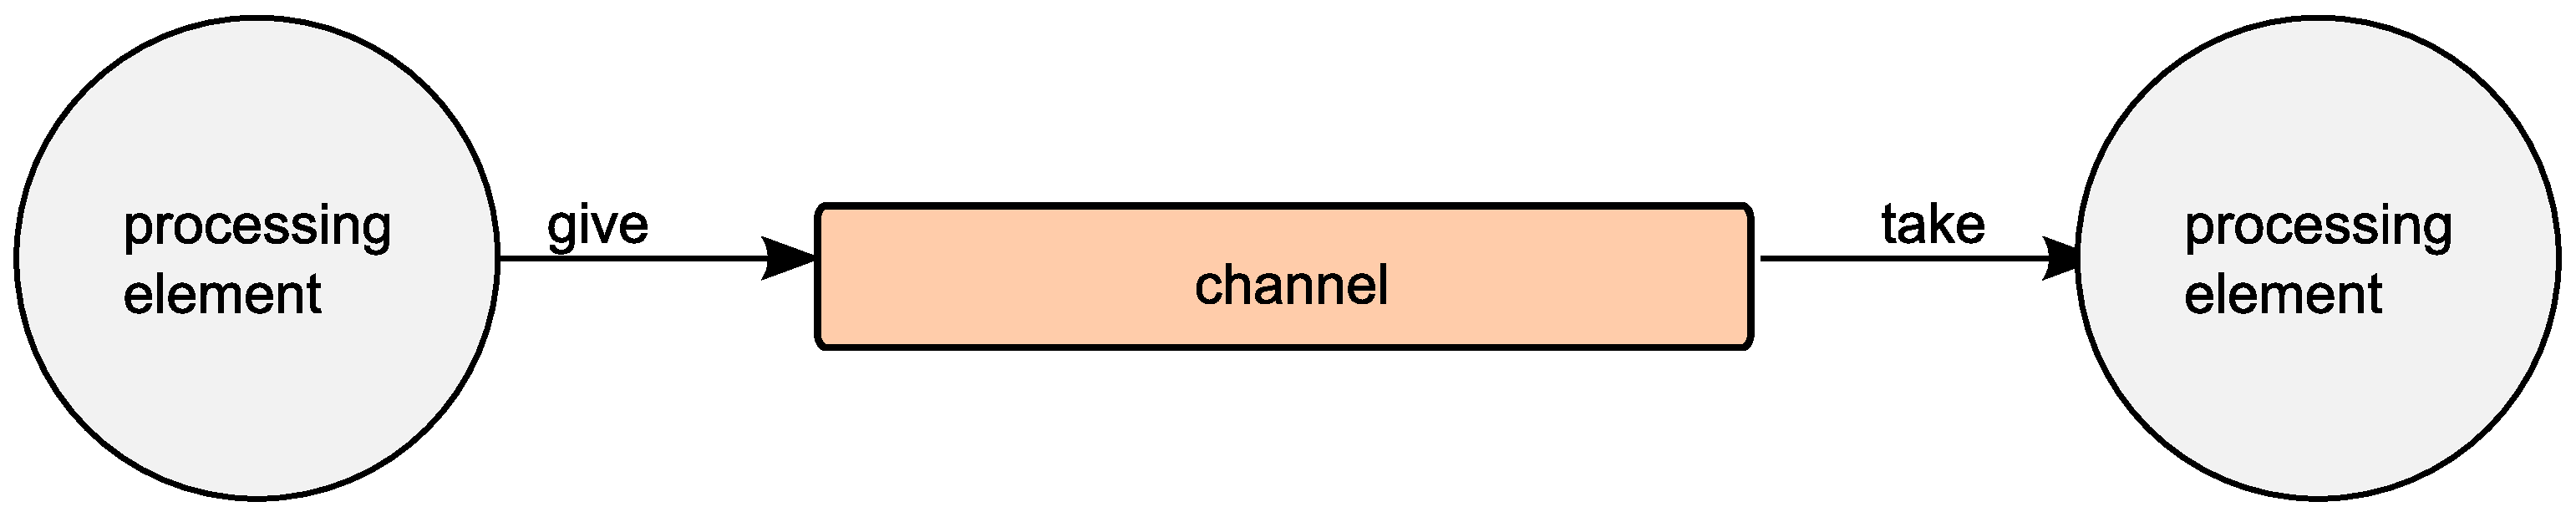
\includegraphics[width=\textwidth]{chapters/gcol/figs/cml_exchange.eps}
    \caption{In \gls{cml}, logical processing elements synchronously exchange values over channels.  When one processing element offers to give a value on a channel, and another offers to take a value on the same channel, they ‘rendezvous’ and exchange the value as a passed message.}
    \label{fig:cml_exchange}
\end{figure}

We were interested in exploring \gls{cml} as another methodology to use for simulating \gls{ps} where communication is involved.  For a first experiment, we chose to implement Gheorghe \textit{et al.}'s 3-colouring problem solution from \cite{Gheorghe2013}, as it involves communication between compartments but is relatively low-complexity and thus appears to be suitable for a first attempt.

We chose to use the programming language \fsharp{} with the library Hopac,\footnote{\url{https://github.com/Hopac/Hopac}} which is modelled on \gls{cml} and follows it closely.\footnote{The final program can be found at \url{https://github.com/jcoo092/acmc2018}}  `Record' types are used to represent the individual compartments described in \cite{Gheorghe2013}.  The program then advances through multiple steps, applying the rules (encoded as functions that operate on the record types) in accordance with \cite{Gheorghe2013}.  Finally, once a solution is found, or found not to be possible, that is communicated to the environment.

Insofar as possible, our implementation has been created to follow the algorithm described in \cite{Gheorghe2013} faithfully, and thus perhaps is not optimal in its efficiency, as an idiomatic specification of a Simple Kernel P~system does not necessarily match to the idiomatic or efficient form of an \fsharp{} program.  That is, we have written the program to prioritise staying as close to the original \gls{skps} model as possible, rather than writing the program to suit the strengths and typical style of the host language.  Consequently the efficiency of the program may be worse than it could be otherwise.  

Ultimately, however, this example is relatively trivial and involves little communication, and therefore does not test the use of \gls{cml} significantly.  Much of the operation of the algorithm in fact does not involve communication between different compartments/processing elements at all.  Instead, it is primarily based in the evolution of objects contained within the compartments, with minimal communication between compartments at the end.  While that is highly effective in \gls{ps} \cite{Paun2008}, it would be interesting to see the results of using \gls{cml} for other problems where synchronous communication\footnote{Note that, while \gls{cml} uses synchronous communication by default, it is relatively simple to implement asynchronous communication also using it \cite{Reppy2007}.} is a much bigger part of the evolution of the system.

We do note here that, in common with most ad-hoc simulations, while our implementation is reasonably successful, it is the case that it is not particularly customisable, and the code as written does not comport as precisely to the appearance of the theoretical rules of the \gls{skps}~system as the \gls{plingua} version created for \cite{Gheorghe2013} does.  Neither does ours have any form of verification or invariant detection, as provided by \gls{mecosim} \cite{Perez-Hurtado2010} and Spin \cite{Ben-Ari2008,Lefticaru2011}.  We suggest that it would be worthwhile to pursue future work that seeks to improve one implementation/simulation by incorporating relevant parts of the other.

\gls{cml} seems to match to \gls{skps} well, but also looks like it might fit well with \gls{tlps} with symport/antiport \cite{Verlan2005} as well perhaps as \gls{tlps} with Channel States \cite{Song2016}, and Generalized Communicating \gls{ps} with minimal interaction rules \cite{Csuhaj-Varju2011}.  It would also appear to be a good fit for Spiking Neural \gls{ps} \cite{Ionescu2006}, though \gls{cml} would probably be `overkill' for those systems when running on a shared-memory system.  In general, any variant of \gls{ps} which heavily uses synchronous communication between different cells/neurons/non-nested membranes/etc. over well-defined channels may be amenable to a \gls{cml} implementation.

Technically, the base form of \gls{cml} would only support antiport (i.e. one-way synchronous communication), but it is fairly simple to build two-way communication on top of it \cite[ch.~6]{Reppy2007}.  We have not attempted to model other systems yet, however.

\subsection{Simulation results}
We recorded our program's running time on a number of differing graphs, with red, green and blue as our set of colours with which to colour the graphs.  The desktop computer used for these simulations has a four-core 3.6GHz Intel Core i7-7700 CPU, with 16GB of RAM, running Windows 10, build number 10.0.17134.228.  Our \fsharp{} programs were run on .NET Core 2.1.4, while \gls{mecosim} was run on Java version 8, build 1.8.0\_201-b09.

Firstly, we used the graph shown in Figure 2 of \cite{Gheorghe2013}, presented in this paper as \autoref{fig:gheorghefig2}, which took 2.6s to process.  In keeping with that paper and following its definition of \(G(N,q)\), where \(G(N,q)\) is used to represent a graph of \(N\) nodes with all other nodes connected only to node \(q\) in a hub-and-spoke formation,\footnote{Note that this is different to the random graphs that are also commonly denoted by this notation.} we also tested the graphs \(G(10,1)\) and \(G(10,10)\) (see \autoref{fig:gs}), finding that it requires 0.3s for each.  We also decided to test our simulation using the classic Petersen graph, shown in \autoref{fig:petersen}, and found that it too required approximately 0.3s.

\begin{figure}
    \centering
    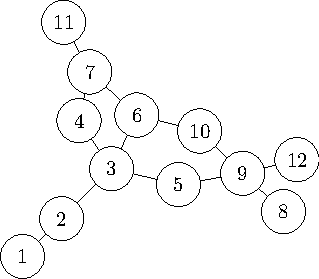
\includegraphics[width=0.65\textwidth]{chapters/gcol/figs/gheorghe-figure-2-figure0.pdf}
    \caption{\label{fig:gheorghefig2}A reproduction of Figure 2 from \cite{Gheorghe2013}.  Although this figure and Figure 2 in \cite{Gheorghe2013} are visually distinct, the graphs are isomorphic.}
\end{figure}

\begin{figure}
    \centering
    \begin{subfigure}[b]{0.35\textwidth}
        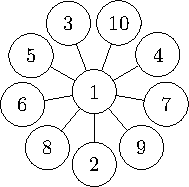
\includegraphics[width=\textwidth]{chapters/gcol/figs/g-10-1.pdf}
        \caption{\label{fig:g-10-1}\(G(10,1)\)}
    \end{subfigure}
    \hfill
    \begin{subfigure}[b]{0.35\textwidth}
        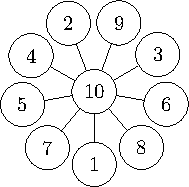
\includegraphics[width=\textwidth]{chapters/gcol/figs/g-10-10.pdf}
        \caption{\label{fig:g-10-10}\(G(10,10)\)}
    \end{subfigure}
    \caption[Graphs representing \(G(10,1)\) and \(G(10,10)\)]{\label{fig:gs}Graphs representing (a) \(G(10,1)\) and (b) \(G(10,10)\), as described in \cite{Gheorghe2013}, where the first number represents the size of the graph, and the second number represents the label of the centre node of the graph, with all other nodes connected only to that node.}
\end{figure}

\begin{figure}
    \centering
    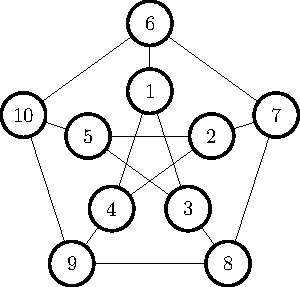
\includegraphics[width=0.45\textwidth]{chapters/gcol/figs/petersen-figure0.pdf}
    \caption{\label{fig:petersen}The classic Petersen graph, with nodes labelled 1 to 10.}
\end{figure}

We further ran our simulation on some complete graphs.  For a complete graph of \(N = 10\), the algorithm again requires 0.3s.  We then tried it on a complete graph of \(N = 20\), but the test had to be aborted after a matter of minutes due to the computer running out of memory.  We then recorded running times of 0.83s, 2.6s, 8.88s, 26.6s and 84s for \(N = 11, 12, 13, 14\) and \(15\), respectively.  Given that we observed significant jumps in memory use in the course of running the larger graphs, it appears that the major cause of the rapid slowdown is likely to do with frequent ad-hoc memory allocations and de-allocations, though we have not profiled this fully.

% Based on the nearly-identical running times for the different graphs of size \(N = 10\), we conclude that our implementation is entirely invariant to the edges of the graph, and the running time depends only on the total number of nodes \(N\).  This is to be expected, since the program as written works as a simple brute-force exploration of the potential solution space.

Gheorghe \textit{et al.} state \cite[p.~828]{Gheorghe2013} that in the latest version of \gls{plingua} at the time of writing, a strategy of eliminating compartments for which there can be no further rule applications is employed.  Using said strategy, results are typically achieved quite quickly.  It has the effect of pruning the search space, and reduces the total running time in some instances to just one-fifth of the running time of the simulation without such dead-compartment-elimination.

Our program does not choose which compartments to operate upon in the same fashion, but we note that applying the colour guard on rule \(r_{2,2n+1}\) of the \gls{skps}~system throughout the process results in the pruning of compartments which already contain invalid results and thus can be eliminated safely, so in order to achieve the same effect as with \gls{plingua}'s strategy, we apply this guard in the course of applying rule \(r_{2,2n+1}\) and use the result to filter out all invalid compartments.  Doing this reduces the evaluation of complete graphs to around 60 milliseconds or slightly more, since every compartment in them can always be entirely eliminated once colours have been assigned to four nodes.  It also reduces the running time of \autoref{fig:gheorghefig2} to around 0.25s, and the Petersen graph, \(G(10,1)\) and \(G(10,10)\) to 0.1s.

\subsubsection{Comparison with original results}

\autoref{tab:timings} compares the timing results of the simulations reported in \cite{Gheorghe2013}, as well as the results of using \gls{mecosim}\footnote{The latest version of \gls{mecosim} available from \url{http://www.p-lingua.org/mecosim/} as at 10 January 2019 was used.} \cite{Perez-Hurtado2010} to re-run the same simulations locally on the same computer used to time our solution, along with the timing results mentioned above.

\begin{table}
\centering
\caption{Comparison of recorded timings between \cite{Gheorghe2013} and this work.  All measurements are in seconds, unless otherwise stated.  Where more than one result was reported in \cite{Gheorghe2013} for the same graph, the shortest running time has been included here.}
\label{tab:timings}
%\resizebox{\textwidth}{!}{%
\begin{tabular}{@{}lcccc@{}}
\toprule
Graph       & \begin{tabular}[c]{@{}c@{}}\gls{plingua}\\ (original)\end{tabular} & \begin{tabular}[c]{@{}c@{}}\gls{plingua}\\ (local)\end{tabular} & CML   & \begin{tabular}[c]{@{}c@{}}CML with\\ pruning\end{tabular} \\ \midrule
Fig. 2      & N/A                                                           & 17.0                                                           & 2.6  & 0.25                                                 \\
Petersen    & N/A                                                           & 1.5                                                       & 0.3  & 0.1                                                       \\
G(10,1)     & 7                                                            & 2.6                                                           & 0.3  & 0.1                                                       \\
G(10,10)    & \textgreater 4 min                             & N/A                                                           & 0.3  & 0.1                                                       \\
Complete 11 & 5                                                            & 0.15                                                           & 0.83 & .06                                                       \\
Complete 12 & 5                                                            & 0.15                                                           & 2.6  & .06                                                       \\
Complete 13 & 5                                                            & 0.15                                                           & 8.88 & .06                                                       \\
Complete 14 & 5                                                            & 0.15                                                           & 26.6 & .06                                                       \\
Complete 15 & 5                                                            & 0.15                                                           & 84   & .06                                                       \\ \bottomrule
\end{tabular}%
%}
\end{table}

Our attempts to run the simulation of \(G(10,10)\) repeatedly failed with an out-of-memory error.  We are unsure as to why this should be the case, given that in the other instances our executions of the \gls{mecosim} \gls{skps} simulations achieved lower runtimes than those of the original paper.  We believe that, execution of \(G(10,10)\) notwithstanding, the overall improvements in runtime of the \gls{skps} sytems are likely due to a combination of the computer used locally being more recent and thus likely more powerful, and improvements in the underlying \gls{mecosim} and \gls{plingua} software.

Further, we find it odd that two functionally identical graphs, \(G(10,1)\) and \(G(10,10)\), would have such dramatically different run time behaviours when running in \gls{mecosim} -- seen in both the original and our local results.  We speculate this might be due to an unusual performance bug hidden deep within \gls{mecosim}, though we have not investigated this further.

These results appear to suggest that our final implementation generally provides superior results with regards to running time, though it must be emphasised that we have not tested a particularly wide variety of scenarios.  We speculate that the scenarios that would provide the `worst' running time will likely be those that have a moderate level of connectedness in the graph.  Highly connected graphs will likely see many potential paths eliminated early due to frequent occurrences of colour conflicts, while graphs with few connections will not have many potential paths to explore.

Our results and those of the \gls{mecosim} simulations are not \emph{completely} comparable, however.  Our solution was programmed directly to follow the \gls{skps} system's rules, whereas the \gls{mecosim} solution was specified as the \gls{skps}~system rules in \gls{plingua}, with the operation of the computer simulation carried out by \gls{mecosim}.  This difference between `ad-hoc' and `general' simulation means that one would expect to see our simulation achieve better results from the outset, as overheads that accompany a general simulation implementation can be avoided.\footnote{One could see ad-hoc as being akin to running a program compiled to native instructions, while using a general simulation is similar in principle to running a program in an interpreter.  The latter is typically simpler to work with and more portable, but comes with overheads that slow down execution.}  \gls{mecosim} is an excellent tool and combined with \gls{plingua} it provides a valuable service to the Membrane Computing community, in that it allows researchers to validate their systems and rulesets while staying close to their mathematical descriptions, and without having to delve into the details of implementing a given algorithm in code.  See further \cite{Perez-Hurtado2018} for more of a discussion on ad-hoc versus general simulations, and the beginnings of a substantial narrowing of the differences between the two.